\section*{Распределение организаций по отраслям}

Каждая организация специализируется на какой-либо отрасли. Для того чтобы понять, какая отрасль является самой популярной на данной момент вычислим число организаций, работающих в этой отрасли (листинг \ref{industryorg}).

Результаты представлены в виде пузырьковой диаграммы (рис. \ref{industryorg}).

Используются:
\begin{itemize}
    \item Объект: \href{https://www.wikidata.org/wiki/Q4830453}{business enterprise (Q4830453)} (коммерческая организация).
    \item Свойство: \href{https://www.wikidata.org/wiki/Property:P452}{industry (P542)} (отрасль).
\end{itemize}

\begin{lstlisting}[language=SPARQL,label=industryorg,caption=Пузырьковая диаграмма распределения организаций по отраслям]
#enterprise industry ranking
#defaultView:BubbleChart
SELECT ?industry ?company (count(*) as ?count)
WHERE 
{
    ?org wdt:P31 wd:Q4830453.
    ?org wdt:P452 ?industry.
    OPTIONAL {
		?industry rdfs:label ?company
		filter (lang(?company) = "en")
	}
}
GROUP BY ?industry ?company
ORDER BY DESC(?count) ASC(?company)
\end{lstlisting}

\href{https://query.wikidata.org/#%23enterprise%20industry%20ranking%0A%23defaultView%3ABubbleChart%0ASELECT%20%3Findustry%20%3Fcompany%20%28count%28%2a%29%20as%20%3Fcount%29%0AWHERE%20%0A%7B%0A%20%20%20%20%3Forg%20wdt%3AP31%20wd%3AQ4830453.%0A%20%20%20%20%3Forg%20wdt%3AP452%20%3Findustry%20.%0A%20%20%20%20OPTIONAL%20%7B%0A%09%09%3Findustry%20rdfs%3Alabel%20%3Fcompany%0A%09%09filter%20%28lang%28%3Fcompany%29%20%3D%20%22en%22%29%0A%09%7D%0A%7D%0AGROUP%20BY%20%3Findustry%20%3Fcompany%0AORDER%20BY%20DESC%28%3Fcount%29%20ASC%28%3Fcompany%29%0A}{SPARQL-запрос}, 864 записи.

Проанализировав данную диаграмму (рис. \ref{industrygraph}), можно сделать вывод о количестве организаций, специализирующихся в той или иной отрасли. На основе (рис. \ref{industrygraph}) построим таблицу, включающую 5 самых популярных отраслей.
 
\begin{table}[h]
\centering
\begin{tabular}{|l|l|}
\hline
\textbf{Название отрасли} & \textbf{Количество организаций} \\
\hline
Автомобильная промышленность & 1149 \\	
\hline
Розничная торговля & 843 \\
\hline
Телекоммуникации & 648 \\
\hline
Видеоигры & 633 \\
\hline
Обрабатывающая промышленность & 506 \\
\hline
\end{tabular}
\caption{Топ-5 самых популярных отраслей}
\label{topindustry}
\end{table}


\begin{figure}[h]
	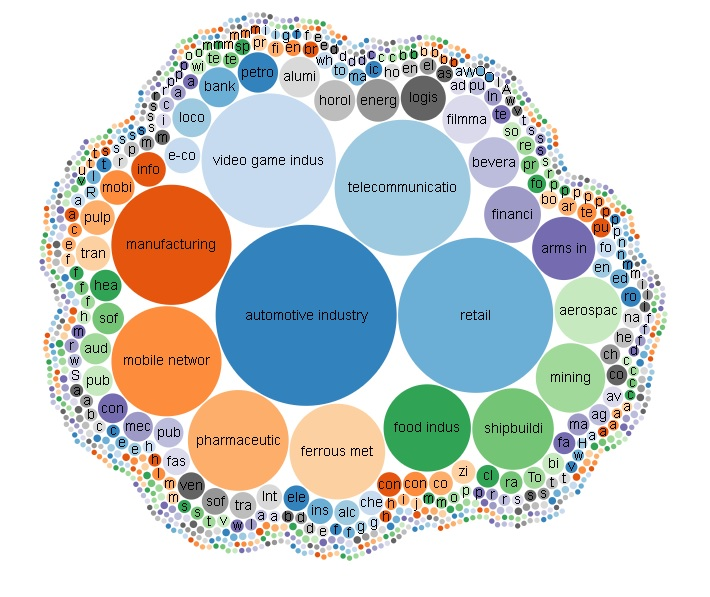
\includegraphics[scale=2.2]{branch/branch.png}
	\centering
	\caption{Пузырьковая диаграмма организаций мира по отраслям}
	\centering
	\label{industrygraph}
\end{figure}

\newpage

Ответим на следующий вопрос: \enquote{Какие и сколько отраслей существуют в России?} с помощью запроса, представленного на листинге \ref{rusidustry}.

\begin{lstlisting}[language=SPARQL,label=rusidustry,caption=Запрос на построение пузырьковой диаграммы распределения организаций по отраслям в России]
#enterprise industry ranking in Russia
#defaultView:BubbleChart
SELECT ?industry ?company (count(*) as ?count) 
WHERE 
{
    ?org wdt:P31 wd:Q4830453.
    ?org wdt:P452 ?industry. #industry
    ?org wdt:P17 wd:Q159. #Russia country
    OPTIONAL {
		?industry rdfs:label ?company
		filter (lang(?company) = "en")
	}
}
GROUP BY ?industry ?company
ORDER BY DESC(?count) ASC(?company)
\end{lstlisting}

\href{https://query.wikidata.org/#%23enterprise%20industry%20ranking%0A%23defaultView%3ABubbleChart%0ASELECT%20%3Findustry%20%3Fcompany%20%28count%28%2a%29%20as%20%3Fcount%29%20%0AWHERE%20%0A%7B%0A%20%20%20%20%3Forg%20wdt%3AP31%20wd%3AQ4830453.%0A%20%20%20%20%3Forg%20wdt%3AP452%20%3Findustry%20.%0A%20%20%20%20%3Forg%20wdt%3AP17%20wd%3AQ159.%20%23Russia%20country%0A%20%20%20%20OPTIONAL%20%7B%0A%09%09%3Findustry%20rdfs%3Alabel%20%3Fcompany%0A%09%09filter%20%28lang%28%3Fcompany%29%20%3D%20%22en%22%29%0A%09%7D%0A%7D%0AGROUP%20BY%20%3Findustry%20%3Fcompany%0AORDER%20BY%20DESC%28%3Fcount%29%20ASC%28%3Fcompany%29%0A}{SPARQL-запрос}, 60 записей.
	
\begin{figure}[h]
	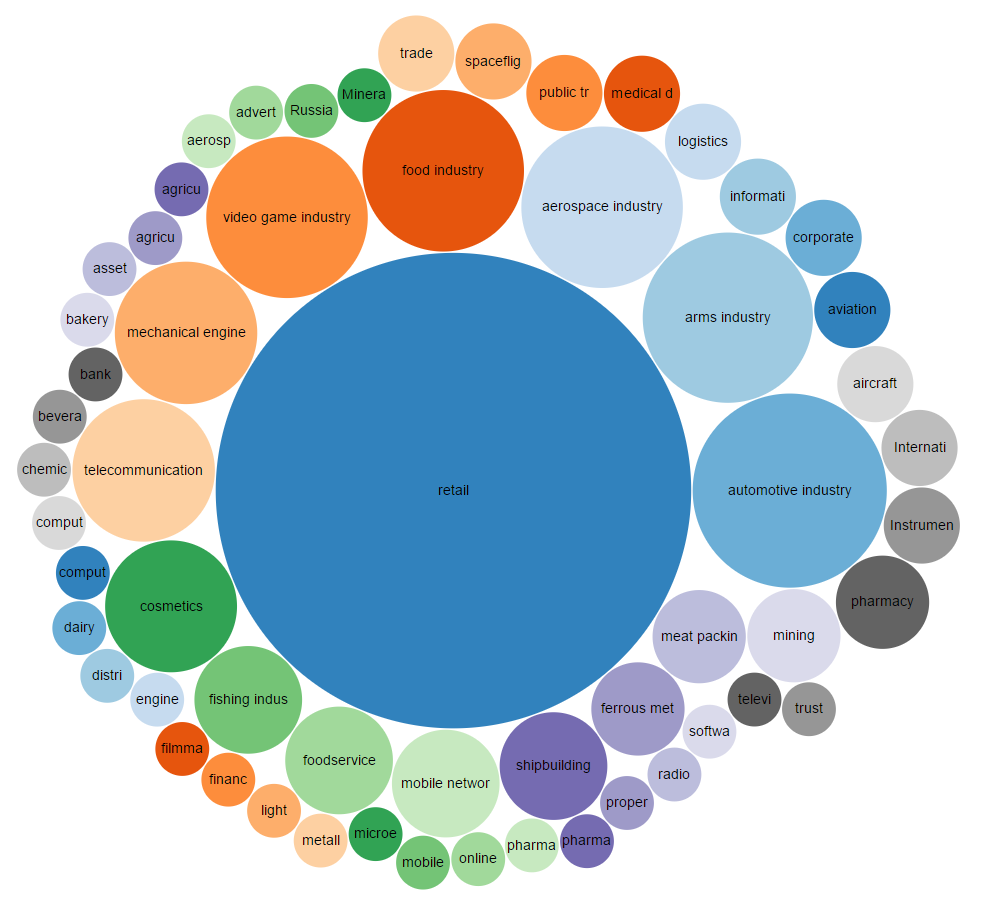
\includegraphics[scale=0.5]{rusdia.png}
	\centering
	\caption{Пузырьковая диаграмма организаций России по отраслям}
	\centering
	\label{industrygraph2}
\end{figure}

\begin{table}[h]
\centering
\begin{tabular}{|l|l|}
\hline
\textbf{Название отрасли} & \textbf{Количество организаций} \\
\hline
Розничная торговля & 78 \\
\hline
Автомобильная промышленность & 13 \\	
\hline
Оружейная промышленность & 10 \\
\hline
Аэрокосмическая промышленность & 9 \\
\hline
Видеоигры & 9 \\
\hline
\end{tabular}
\caption{Топ-5 самых популярных отраслей в России}
\label{topindustryrus}
\end{table}

Из таблицы \ref{topindustryrus} делаем вывод, что такая отрасль, как розничная торговля, в России существенно преобладает над остальными. Если количество организаций в этой области достигает 78, то в следующей по счету отрасли (автомобильной промышленности) работает только 13 организаций.

Для сравнения России построим список существующих отраслей какой-нибудь другой страны , например, Норвегии (листинг \ref{norwayorgs}).

\begin{lstlisting}[language=SPARQL,label=norwayorgs,caption=Диаграмма распределения организаций по отраслям в Норвегии]
#enterprise industry ranking in Norway
#defaultView:BubbleChart
SELECT ?industry ?company (count(*) as ?count) 
WHERE 
{
    ?org wdt:P31 wd:Q4830453.
    ?org wdt:P452 ?industry.
    ?org wdt:P17 wd:Q20. #Norway country
    OPTIONAL {
		?industry rdfs:label ?company
		filter (lang(?company) = "en")
	}
}
GROUP BY ?industry ?company
ORDER BY DESC(?count) ASC(?company)
\end{lstlisting}

\href{https://query.wikidata.org/#%23enterprise%20industry%20ranking%20in%20Norway%0A%23defaultView%3ABubbleChart%0ASELECT%20%3Findustry%20%3Fcompany%20%28count%28%2a%29%20as%20%3Fcount%29%20%0AWHERE%20%0A%7B%0A%20%20%20%20%3Forg%20wdt%3AP31%20wd%3AQ4830453.%0A%20%20%20%20%3Forg%20wdt%3AP452%20%3Findustry%20.%0A%20%20%20%20%3Forg%20wdt%3AP17%20wd%3AQ20.%20%23Norway%20country%0A%20%20%20%20OPTIONAL%20%7B%0A%09%09%3Findustry%20rdfs%3Alabel%20%3Fcompany%0A%09%09filter%20%28lang%28%3Fcompany%29%20%3D%20%22en%22%29%0A%09%7D%0A%7D%0AGROUP%20BY%20%3Findustry%20%3Fcompany%0AORDER%20BY%20DESC%28%3Fcount%29%20ASC%28%3Fcompany%29%0A}{SPARQL-запрос}, 41 запись.

В Норвегии преобладающей отраслью является \href{https://www.wikidata.org/wiki/Q187939}{manufacturing} (производство).